\begin{exo}
	On a représenté ci-dessous quatre cibles avec l'impact de cinq flèches tirées à l'arc. Chaque couronne a un rayon de 1 unité.

	\begin{center}
		\renewcommand{\arraystretch}{2}
		\begin{tabular}{cc}
			% Cible 1 (Haut-Gauche)
			\begin{minipage}{0.2\textwidth}
				\centering
				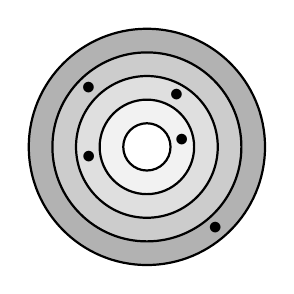
\begin{tikzpicture}[scale=0.3]
					\draw[fill=gray!60,thick] (0,0) circle (5);
					\draw[fill=gray!40, thick] (0,0) circle (4);
					\draw[fill=gray!25, thick] (0,0) circle (3);
					\draw[fill=gray!10, thick] (0,0) circle (2);
					\draw[fill=white, thick] (0,0) circle (1);
					% Impacts
					\node at (135:3.5) {$\bullet$};
					\node at (60:2.5) {$\bullet$};
					\node at (10:1.5) {$\bullet$};
					\node at (190:2.5) {$\bullet$};
					\node at (-50:4.5) {$\bullet$};
				\end{tikzpicture}
			\end{minipage} &
			% Cible 2 (Haut-Droite)
			\begin{minipage}{0.2\textwidth}
				\centering
				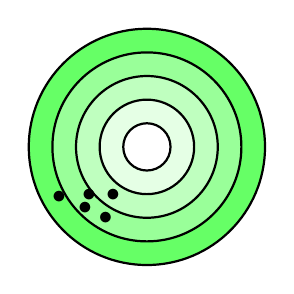
\begin{tikzpicture}[scale=0.3]
					\draw[fill=green!60,thick] (0,0) circle (5);
					\draw[fill=green!40, thick] (0,0) circle (4);
					\draw[fill=green!25, thick] (0,0) circle (3);
					\draw[fill=green!10, thick] (0,0) circle (2);
					\draw[fill=white, thick] (0,0) circle (1);
					% Impacts groupés en bas à gauche
					\node at (210:4.3) {$\bullet$};
					\node at (225:3.7) {$\bullet$};
					\node at (240:3.5) {$\bullet$};
					\node at (220:3.2) {$\bullet$};
					\node at (235:2.5) {$\bullet$};
				\end{tikzpicture}
			\end{minipage}
			\\~\vspace{-6mm}\\
			% Cible 3 (Bas-Gauche)
			\begin{minipage}{0.2\textwidth}
				\centering
				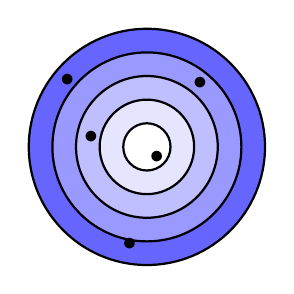
\begin{tikzpicture}[scale=0.3]
					\draw[fill=blue!60,thick] (0,0) circle (5);
					\draw[fill=blue!40, thick] (0,0) circle (4);
					\draw[fill=blue!25, thick] (0,0) circle (3);
					\draw[fill=blue!10, thick] (0,0) circle (2);
					\draw[fill=white, thick] (0,0) circle (1);
					% Impacts
					\node at (140:4.4) {$\bullet$};
					\node at (50:3.5) {$\bullet$};
					\node at (170:2.4) {$\bullet$};
					\node at (-100:4.2) {$\bullet$};
					\node at (-45:0.6) {$\bullet$};
				\end{tikzpicture}
			\end{minipage} &
			% Cible 4 (Bas-Droite)
			\begin{minipage}{0.2\textwidth}
				\centering
				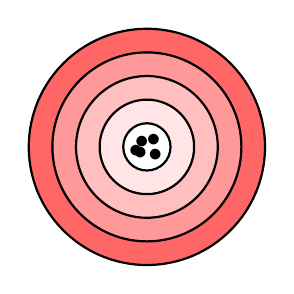
\begin{tikzpicture}[scale=0.3]
					\draw[fill=red!60,thick] (0,0) circle (5);
					\draw[fill=red!40, thick] (0,0) circle (4);
					\draw[fill=red!25, thick] (0,0) circle (3);
					\draw[fill=red!10, thick] (0,0) circle (2);
					\draw[fill=white, thick] (0,0) circle (1);
					% Impacts au centre (dans le cercle de rayon 1)
					\node at (45:0.4) {$\bullet$};
					\node at (135:0.3) {$\bullet$};
					\node at (-45:0.5) {$\bullet$};
					\node at (-135:0.4) {$\bullet$};
					\node at (200:0.5) {$\bullet$};
				\end{tikzpicture}
			\end{minipage}
		\end{tabular}
	\end{center}

	\vspace{0.4cm}

	Pour chaque tireur, on considère la distance de chaque flèche au centre de la cible.

	\begin{enumerate}
		\item Associer chaque couple (moyenne ; écart-type) à chaque cible : $(2,84\ ;\ 0,97)$ ; $(0,79\ ;\ 0,19)$ ; $(3,33\ ;\ 0,55)$ ; $(3,21\ ;\ 1,42)$.
		\item Associer chacun des quatre tireurs à une cible : un tireur expérimenté, deux tireurs débutants et un tireur ayant mal réglé son viseur.
	\end{enumerate}
\end{exo}
